% ------------------------------------
% INTRODUCTION
% ------------------------------------
\section{Introduction}
\label{sec:introduction}
In recent years computing is becoming more ubiquitous in the physical world. This
notion of ubicomp was introduced by Weiser \cite{weiser1999origins}, where the concept of
smart environment was defined as ``\textit{a physical world richly and invisibly
interwoven with sensors, actuators, displays, and computational elements, embedded
seamlessly in the everyday objects of our lives and connected through a continuous network}''.
Through the years, technology advances such as the creation of the Internet contributes
to achieving the ubicomp's vision which enables individual devices to communicate between
themselves from any part of the world \cite{gubbi2013internet}. In Weiser's vision of
ubiquitous computing, information seamlessly moves in and out of attention as automation
gives way to human interaction \cite{weiser1991computer}.\\

The progress towards ubiquitous computing has been slower than expected \cite{greenfield2010everyware},
another approaches for ubiquitous computing that constrasts with Weiser vision becomes relevant.
Rogers' proposes an approach which focuses in designing technologies for engaging user
experiences that in a creative and constructive way, extend the peoples' capabilities \cite{rogers2006moving}.
Rogers points that ubiquitous technologies can be developed not only for individuals,
but for particular domains that can be set up and customized by an organization according
its needs, such as agriculture, retailing and logistics.\\

The main difference between Weiser's and Rogers' vision concerns with the user experience.
In Weiser point of view computers take the initiative to act on people's behalf \cite{tennenhouse2000proactive},
while in Rogers vision is not the computer that is proactive, the user assumes that role.\\

Actually, Weiser vision is close to becoming reality thanks to the Internet of Things
and Cloud Computing \cite{caceres2012ubicomp}. This world where things are connected
through a continuous network is a vision thats represents the Internet of Things (IoT).
In this vision, physical items are continuously connected to the virtual world and can
act as remotely physical access points to Internet Services. The Internet of Things would
make computing truly ubiquitous \cite{mattern2010internet}.\\

A common scenario where the Internet of Things paradigm is applied are smart environments \cite{atzori2010internet},
which in this document are designated as smart places. In the context of this work,
a smart place can be defined as an ecosystem composed by smart objects such as RFID
tags and sensors, that are able to acquire knowledge about this environment and also to
adapt this inhabitants in order to improve their experience in that environment \cite{cook2004smart}.\\

An example of a smart place is a smart warehouse. In the smart warehouse, products and objects
are identified with RFID tags. These tags can be used to tracking the objects inside the warehouse.
To perform the tracking of the objects, the smart warehouse must have an IoT application that process
the data generated by the objects. This application also allow that managers monitor the warehouse.
For instance, is possible to monitor the objects that enters and leaves the warehouse.
To monitoring the objects in the warehouse, the IoT application must be able to identify
the tagged objects. In the case of RFID tagged objects, the EPC Framework provides a complete
support to perform the traceability of objects, as well the awareness of its status and
current location \cite{atzori2010internet}.\\

In particular, the deployment of IoT applications in the smart warehouse is a challenge today
due the heterogeneity of the smart objects that are present in a smart place and also
because the required infrastructure. In order to decrease the complexity of the deployment
of an IoT application in a smart place, the Cloud computing paradigm allows the virtualization
of the required physical infrastructure. Nowadays the server infrastructure needed by IoT
applications can be virtualized by Cloud providers, which gives more flexibility and reduces
the costs in the deployment of an IoT application.\\

Therefore, another challenge concerns the heterogeneity of a smart place, more precisely the variety of
smart objects that can be inside of a given place. Many of these objects uses different communication
protocols and drivers to communicate with devices, thus the configuration of this objects
must be manually handled, which makes the integration of these objects in the deployment of
IoT applications in a smart place an inefficient process.\\
% -------------------------------------
% INTERNET OF THINGS
% -------------------------------------
\subsection{Internet of Things}
\label{sub:internet_of_things}
The Internet of Things is a concept in which the virtual world of information
technology integrates seamlessly with the real world of physical things \cite{Uckelmann:2011:AIT:2018904}.
Through the amount of computer and network devices available nowadays, facts about
the real world becomes accessible to business and everyday use cases.\\

A more precise definition of the Internet of Things was formulated in the Strategic
Research Agenda of the Cluster of European Research Projects on the Internet of Things (CERP-IoT 2009):\\

``\textit{In the IoT, `things' are expected to become active participants in business,
information and social processes where they are enabled (...) by exchanging data
and information  sensed about the environment, while reacting autonomously to the
`real/physical world' events and influencing it by running processes that trigger
actions and create services with or without direct human intervention. Interfaces
in the form of services facilitate interactions with these `smart things' over the
Internet (...) taking into account security and privacy issues.}''\\

Internet of Things will enable a more convenient life for people. One of the expectations
of IoT concerns with providing services to the end-users through common objects, in that way
products will be able to provide recommendations for use and maintenance instructions, supply warranty
information or point to related products.\\

Recently, IoT became relevant to industry and end-users \cite{Uckelmann:2011:AIT:2018904},
mainly because the reduction of cost and  miniaturization of technologies used in IoT applications,
such as RFID, sensor networks, NFC and  wireless communication. Technologies like these allows
the detection of status of things, which  together with collection and processing of detailed
data, allows the creation of an interactive  and responsive network with huge potential
for citizens, consumers, business to gather immediate responses to events that occurs
in the real world \cite{Uckelmann:2011:AIT:2018904}.\\

Using these technologies, IoT can provide access to more detailed information, which results
that the level of analysis can be performed in a large-scale perspective, as well in a
small-scale perspective. But IoT is more than a tool for managing processes more
efficiently and more effectively. Another expectation of IoT concerns with real-world
awareness provided to information systems \cite{mattern2010internet}. An example is logistics
applications, by the use of RFID, companies can react promptly to relevant physical events,
and then manage their processes in a better way, typically increasing efficiency and
reducing costs.

% ---------------------------------------
% CLOUD COMPUTING
% ---------------------------------------
\subsection{Cloud Computing}
\label{sub:cloud_computing}
Cloud Computing is a paradigm where a computing infrastructure is designated as a \textit{``Cloud"}
from which its resources are available to businesses and users from anywhere in the
world on demand \cite{buyya2009cloud}. This paradigm enables rapid service delivery in
a dynamically scalable and virtualized manner. Actually, clouds are built on top of
modern data centers, that incorporated Infrastructure as a Service (IaaS), Platform as a Service (PaaS)
and Software as a Service (SaaS) \cite{tsai2010service}, as illustrated on Figure \ref{fig:high_level_cloud_view}.\\

Cloud providers, such as Amazon Web Services\footnote{http://www.aws.amazon.com},
Google Cloud Platform\footnote{http://cloud.google.com} and Microsoft Azure\footnote{http://www.azure.microsoft.com/}
offer these services as utilities in a pay-per-use model in which Quality of Service \textit{QoS}
guarantees are offered by means of customized Service Level Agreements (SLAs) \cite{vaquero2008break},
that are negotiated between the customers and the Cloud providers.
% Cloud Computing High-Level View
\begin{figure}[h!]
  \centering
  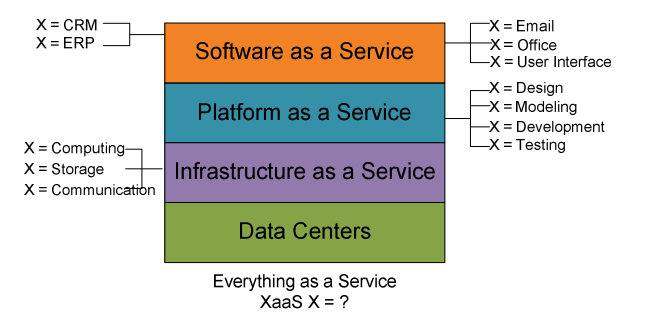
\includegraphics[width=.8\textwidth]{./images/high_level_cloud_view}
  \caption{Hierarchical view of Cloud Computing.}
  \label{fig:high_level_cloud_view}
\end{figure}\\

Data Centers allocates all the hardware that supports the cloud. They consist of
a large number of physical machines that provide redundancy and ensure reliability
in case failures. By using the IaaS pattern, Cloud Computing is able to virtualize
resources as computing power, storage and network connectivity of the data centers.
These computational resources are provisioned on demand in a form of Virtual Machines (VMs)
deployed in a cloud provider data-center \cite{sotomayor2009virtual}. The Cloud can also
be used to assist application design, development, application hosting and testing by providing
a development platform, a service pattern is known as PaaS. Another pattern supported by
Cloud Computing is SaaS. That allows that a single piece of software is transferred to millions
of users through a browser \cite{zhang2010cloud}. This pattern is beneficial to both users
and developers. The developers only needs to maintain a single program while the users can
save costs in servers and software.\\

In a global analysis Cloud computing offers several benefits such as high-availability,
high-scalability, flexibility, on-demand service provisioning and reduction of costs.
By converging IoT applications and Cloud computing, it should be possible to take advantage
of all these benefits.
% -----------------------------------------
% CLOUD ORCHESTRATION
% -----------------------------------------
\subsubsection{Cloud Orchestration}
\label{subs:cloud_orchestration}
Due the heterogeneity of IoT applications infrastructure, service management tasks
such as deployment, driver installation and gateway configuration are still handled
manually for each case. In order to reduce the complexity of these tasks, Cloud Orchestration
tools can be used to automate these management tasks. The orchestration can wove the
software components of the application in one piece that can be managed more effectively.
Cloud Orchestration helps to take advantage of the full benefits of Cloud computing by
providing features that can include:
% Orchestration Features
\begin{itemize}
  \item Simplify, automate and optimize service deployment by integrating cloud capabilities
  across heterogeneous environments.
  \item Automated high-scale provisioning and de-provisioning of resources with policy-based tools.
  \item Real-time monitoring of physical and virtual resources.
  \item Selection of Cloud services such as storage and hosting, through a self-service portal.
  \item Real-time monitoring of usage and accounting chargeback capabilities to track and optimize system usage.
\end{itemize}
In addition, orchestration allows significantly reduction of the costs related with labor
and resources, since that manual intervention and management of varied IT services and resources
are not needed. Currently, several tools to performing Cloud Orchestration are available
in the market such as IBM Cloud Orchestrator\footnote{http://www.ibm.com/software/products/en/ibm-cloud-orchestrator},
HP Operations Orchestration\footnote{http://www8.hp.com/us/en/software-solutions/operations-orchestration-it-process-automation}
and GigaSpaces Cloudify\footnote{http://www.gigaspaces.com/cloudify-cloud-orchestration/overview}
and some open-source tools like Ubuntu Juju\footnote{http://www.juju.ubuntu.com}
and OpenTOSCA\footnote{http://www.iaas.uni-stuttgart.de/OpenTOSCA/indexE.php}.\\
% -----------------------------------------
% SMART SPACES ARCHITECTURE
% -----------------------------------------
\subsection{Smart Places Architecture}
\label{sub:smart_places_architecture}
As described before, a smart place is composed by several smart objects that generates
data that is processed by the IoT application. However, to process all that data an
infrastructure is required to support the IoT application. These infrastructure is composed
by RFID tags, sensors, readers and servers, as illustrated in Figure \ref{fig:smart-space}.
Although this infrastructure can support the IoT application in the smart place, this
architecture presents several issues regarding the deployment of the application, the low scalability,
the costs of infrastructure and the maintenance of the same.
% Typical Smart Space Scenario
\begin{figure}[h!]
  \centering
  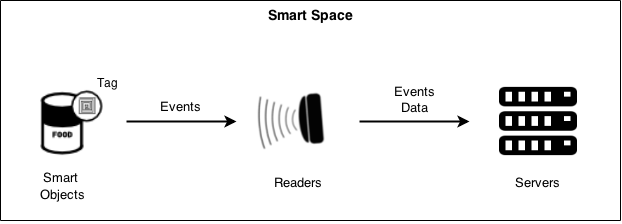
\includegraphics[width=\textwidth]{./images/smart-space}
  \caption{Typical smart place scenario, using RFID technology.}
  \label{fig:smart-place}
\end{figure}\\
By converging the IoT applications with the Cloud computing paradigm the objective is simplify the
smart space architecture by leveraging the required infrastructure by these applications to
the Cloud providers, as illustrated in Figure \ref{fig:smart-space-cloud}, allowing to take
advantage of the benefits offered by Cloud computing (as referenced in \textbf{Section \ref{sub:cloud_computing}}).
% Cloud-based Smart Space Scenario
\begin{figure}
  \centering
  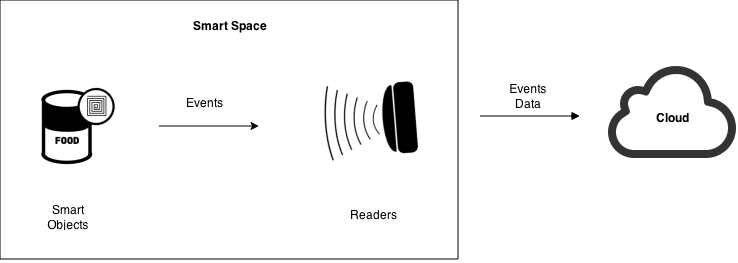
\includegraphics[width=\textwidth]{./images/smart-space-cloud}
  \caption{Cloud-based smart place.}
  \label{fig:smart-place-cloud}
\end{figure}\\
The convergence between the IoT applications and the Cloud allow to simplify the
architecture of the smart place in a significantly way. However, as earlier mentioned
these solution still presents some issues to be resolved, namely the deployment of
the application.
% -----------------------------------------
% OVERVIEW
% -----------------------------------------
\subsection{Overview}
\label{sub:overview}
The remainder of this document is organized as the follows. In Section \ref{sec:objectives}
we describe the problem to be solved as well the main objectives of this work. Section \ref{sec:related_work}
presents the related work in the research area. Then in Section \ref{sec:solution_architecture}
we present a brief description of the state of art solution and propose the architecture
for our solution. In Section \ref{sec:evaluation} the evaluation methodology is described.
Section \ref{sec:conclusion} presents the conclusion. In the appendix a schedule
for the future work is presented.
